%\motto{Use the template \emph{chapter.tex} to style the various elements of your chapter content.}
\chapter{Introducción}
\label{intro} % Always give a unique label
% use \chaptermark{}
% to alter or adjust the chapter heading in the running head

\abstract*{Each chapter should be preceded by an abstract (no more than 200 words) that summarizes the content. The abstract will appear \textit{online} at \url{www.SpringerLink.com} and be available with unrestricted access. This allows unregistered users to read the abstract as a teaser for the complete chapter.
    Please use the 'starred' version of the new \texttt{abstract} command for typesetting the text of the online abstracts (cf. source file of this chapter template \texttt{abstract}) and include them with the source files of your manuscript. Use the plain \texttt{abstract} command if the abstract is also to appear in the printed version of the book.}

\abstract{Each chapter should be preceded by an abstract (no more than 200 words) that summarizes the content. The abstract will appear \textit{online} at \url{www.SpringerLink.com} and be available with unrestricted access. This allows unregistered users to read the abstract as a teaser for the complete chapter. \newline\indent
    Please use the 'starred' version of the new \texttt{abstract} command for typesetting the text of the online abstracts (cf. source file of this chapter template \texttt{abstract}) and include them with the source files of your manuscript. Use the plain \texttt{abstract} command if the abstract is also to appear in the printed version of the book.}

Considere un dominio $\Omega\subset\mathbb{R}^{n}$ y una cantidad de
interés $\bm{U}$ definida para todos los $\bm{x}\in\Omega$.
La cantidad de interés podría ser la concentración de un químico o la
densidad de una población humana, la presión de un fluido o la
temperatura de una cuerda.

La evolución en tiempo de esta cantidad de interés $\bm{U}$
puede ser descrito mediante la observación:
\begin{quote}
    La tasa temporal de cambio de $\bm{U}$ en cualquier subdominio
    fijo $\omega\in\Omega$ es igual a la cantidad total de
    $\bm{U}$ producido o destruido dentro de $\omega$ y el flujo
    de $\bm{U}$ a través de la frontera $\partial\omega$.
\end{quote}
Esta observación se describe matemáticamente como
\begin{equation}\label{eq:integralbalance}
    \diff{}{t}
    \int_{\omega}
    \bm{U}\dl{\bm{x}}=
    -\int_{\partial\omega}
    \bm{F}\cdot\nu\dl{\sigma\left(\bm{x}\right)}+
    \int_{\omega}
    \bm{S}\dl{\bm{x}}.
\end{equation}
donde $\nu$ es la normal unitaria exterior,
$\dl{\sigma\left(\bm{x}\right)}$ es la medida de la superficie,
$\bm{F}$ es el flujo y $\bm{S}$ es la fuente.
Así,~\eqref{eq:integralbalance} es la ecuación integral para la
evolución de la cantidad total de $\bm{U}$ en $\omega$.
\begin{figure}[b]
    \sidecaption
    % Use the relevant command for your figure-insertion program
    % to insert the figure file.
    % For example, with the option graphics use
    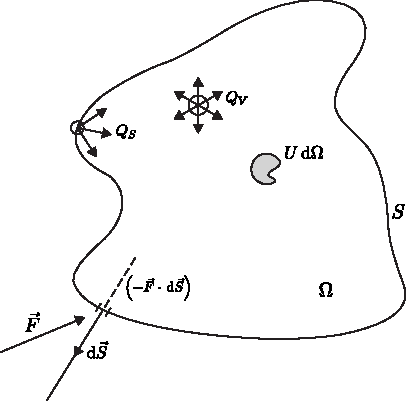
\includegraphics{conservationscheme}
    %
    % If not, use
    %\picplace{5cm}{2cm} % Give the correct figure height and width in cm
    %
    \caption{If the width of the figure is less than 7.8 cm use the
        \texttt{sidecapion} command to flush the caption on the left side of the page.
        If the figure is positioned at the top of the page, align the sidecaption with
        the top of the figure -- to achieve this you simply need to use the optional
        argument \texttt{[t]} with the \texttt{sidecaption} command}
    \label{fig:1}       % Give a unique label
\end{figure}
Simplificamos~\eqref{eq:integralbalance} utilizando el teorema de la
divergencia de Gauß en la integral de superficie para obtener
\begin{equation}\label{eq:integralbalance2}
    \diff{}{t}
    \int_{\omega}
    \bm{U}\dl{\bm{x}}
    +\int_{\omega}
    \operatorname{div}
    \left(\bm{F}\right)\dl{\bm{x}}=
    \int_{\omega}
    \bm{S}\dl{\bm{x}}.
\end{equation}
Dado que~\eqref{eq:integralbalance2} se cumple para cualquier
subdominio $\omega\subset\Omega$,
\begin{equation}\label{eq:balancelaw}
    \forall\left(x,t\right)\in\Omega\times\mathbb{R}_{+}:
    \difcp{\bm{U}}{t}+
    \operatorname{\operatorname{div}
        \left(\bm{F}\right)}=
    \bm{S}.
\end{equation}
La ecuación~\eqref{eq:balancelaw} se llama \emph{ley de balance}.
Frequentemente, el único cambio en $\bm{U}$ proviene de los
flujos y la fuente se fija en cero.
\begin{equation}\label{eq:conservationlaw}
    \forall\left(x,t\right)\in
    \Omega\times\mathbb{R}_{+}:
    \difcp{\bm{U}}{t}+
    \operatorname{\operatorname{div}
        \left(\bm{F}\right)}=
    0.
\end{equation}
La ecuación~\eqref{eq:conservationlaw} se llama
\emph{ley de conservación}, ya que el único cambio en $\bm{U}$
procede de la cantidad que entra o sale del dominio de interés.

\section*{Ejemplos de leyes de conservación}

Algunos ejemplos de leyes de conservación son la ecuación de
transporte escalar, la ecuación de difusión, las ecuaciones de Euler,
la ecuación de Richards y la ecuación Buckley-Leverett.

\subsection*{Ecuación de transporte escalar}

Sea $\bm{U}=U$ la concentración de un contaminante en un río.
Suponga que el río fluye con un campo de velocidad
$\bm{a}\left(\bm{x},t\right)$ y conocemos el campo de
velocidad en todos los puntos del río.
El contaminante es transportado en la dirección de la velocidad, y
así el flujo es $\bm{F}=\bm{a}U$.
Dado que no hay producción ni destrucción del contaminante durante el
flujo, el término fuente en~\eqref{eq:balancelaw} es cero.
La ley de conservación~\eqref{eq:conservationlaw} resulta ser
\begin{equation}
    \difcp{U}{t}+
    \operatorname{div}
    \left(\bm{a}\left(\bm{x},t\right)U\right)=
    0.
\end{equation}

\subsection*{Ecuación de difusión}

Sea $\bm{U}=U$ la temperatura de un bloque metálico.
Suponga que el bloque se calienta por un extremo y se deja enfriar
después, sin aportar ninguna fuente de calor adicional.
El calor se propaga o difunde y la temperatura del bloque se
uniformiza al cabo de un tiempo.
La difusión del calor se rige por la ley de Fick
\begin{equation}\label{eq:ficklaw}
    \bm{F}\left(U\right)=
    -\bm{k}\nabla U.
\end{equation}
Aquí, $\bm{k}$ es el tensor de conductividad del medio.
Sustituyendo~\eqref{eq:ficklaw} en~\eqref{eq:conservationlaw}
resulta ser
\begin{equation*}
    \difcp{U}{t}-
    \operatorname{div}
    \left(\bm{k}\nabla U\right)=
    0.
\end{equation*}

\subsection*{Ecuaciones de Euler}

El aire consiste de un gran número de moléculas.
El movimiento de cada molécula puede seguirse individualmente y
da lugar a un gran número de EDOs.
El sistema EDO resultante es demasiado grande para ser
computacionalmente viable.
En su lugar, se utiliza una descripción macroscópica.
Las variables de interés son: la densidad $\rho$, el campo de
velocidad $u$ y la presión del gas $p$.

\begin{description}
    \item[Conservación de la masa]

    \item[Conservación del momento]

    \item[Conservación de la energía]
\end{description}

\begin{align*}
    \difcp{\rho}{t}+
    \operatorname{div}
    \left(\rho\bm{u}\right)                       & =0. \\
    \difcp{\rho\bm{u}}{t}+
    \operatorname{div}
    \left(\rho\bm{u}\otimes\bm{u}\right)+\nabla p & =0. \\
    \difcp{E}{t}+
    \operatorname{div}
    \left(\left(E+p\right)\bm{u}\right)           & =0.
\end{align*}

\subsection*{Ecuación de Richards}

\subsection*{Ecuación de Buckley-Leverett}

\section{Antecedentes}
\label{sec:1}
Use the template \emph{chapter.tex} together with the document class SVMono (monograph-type books) or SVMult (edited books) to style the various elements of your chapter content conformable to the Springer Nature layout.

\section{Trabajos relacionados}
\section{Modelo de leyes de conservación}
\label{sec:2}
% Always give a unique label
% and use \ref{<label>} for cross-references
% and \cite{<label>} for bibliographic references
% use \sectionmark{}
% to alter or adjust the section heading in the running head

\eject

however, for multiline equations we recommend to use the \verb|eqnarray| environment\footnote{In physics texts please activate the class option \texttt{vecphys} to depict your vectors in \textbf{\itshape boldface-italic} type - as is customary for a wide range of physical subjects.}.
\begin{eqnarray}
    \left|\nabla U_{\alpha}^{\mu}(y)\right| &\le&\frac1{d-\alpha}\int
    \left|\nabla\frac1{|\xi-y|^{d-\alpha}}\right|\,d\mu(\xi) =
    \int \frac1{|\xi-y|^{d-\alpha+1}} \,d\mu(\xi)\qquad  \\
    &=&(d-\alpha+1) \int\limits_{d(y)}^\infty
    \frac{\mu(B(y,r))}{r^{d-\alpha+2}}\,dr \le (d-\alpha+1)
    \int\limits_{d(y)}^\infty \frac{r^{d-\alpha}}{r^{d-\alpha+2}}\,dr
    \label{eq:01}
\end{eqnarray}

\enlargethispage{24pt}

\subsection{Modelo de Burgers}
\label{subsec:2}
Instead of simply listing\index{cross-references} and citations\index{citations} as has already been described in Sect.~\ref{sec:2}.

\begin{quotation}
    Please do not use quotation marks when quoting texts! Simply use the \verb|quotation| environment -- it will automatically be rendered in the preferred layout.
\end{quotation}

\subsection{Buckley-Leverett}

\paragraph{Paragraph Heading} %
Instead of simply listing headings of different levels we recommend to let every heading be followed by at least a short passage of text. Furtheron please use the \LaTeX\ automatism for all your cross-references and citations as has already been described in Sect.~\ref{sec:2}.

\begin{enumerate}
    \item{Livelihood and survival mobility are oftentimes coutcomes of uneven socioeconomic development.}
\end{enumerate}


\subparagraph{Subparagraph Heading} In order to avoid simply listing headings of different levels we recommend to let every heading be followed by at least a short passage of text. Use the \LaTeX\ automatism for all your cross-references and citations as has already been described in Sect.~\ref{sec:2}, see also Fig.~\ref{fig:2}.

Please note that the first line of text that follows a heading is not indented, whereas the first lines of all subsequent paragraphs are.

\begin{itemize}
    \item{Livelihood and survival mobility are oftentimes coutcomes of uneven socioeconomic development, cf. Table~\ref{tab:1}.}
\end{itemize}

\begin{figure}[t]
    \sidecaption[t]
    % Use the relevant command for your figure-insertion program
    % to insert the figure file.
    % For example, with the option graphics use
    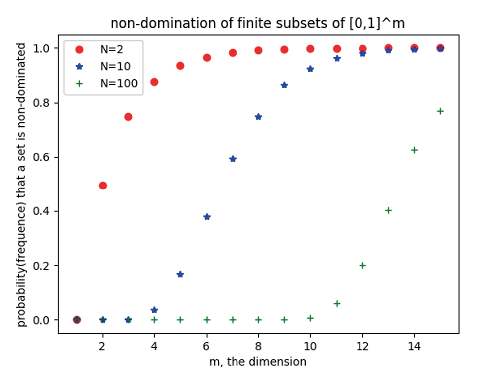
\includegraphics{figure}
    %
    % If not, use
    %\picplace{5cm}{2cm} % Give the correct figure height and width in cm
    %
    \caption{Please write your figure caption here}
    \label{fig:2}       % Give a unique label
\end{figure}

\runinhead{Run-in Heading Boldface Version} Use the \LaTeX\ automatism for all your cross-references and citations as has already been described in Sect.~\ref{sec:2}.

\subruninhead{Run-in Heading Boldface and Italic Version} Use the \LaTeX\ automatism for all your cross-refer\-ences and citations as has already been described in Sect.~\ref{sec:2}\index{paragraph}.

\subsubruninhead{Run-in Heading Displayed Version} Use the \LaTeX\ automatism for all your cross-refer\-ences and citations as has already been described in Sect.~\ref{sec:2}\index{paragraph}.
% Use the \index{} command to code your index words
%
% For tables use
%
\begin{table}[!t]
    \caption{Please write your table caption here}
    \label{tab:1}       % Give a unique label
    %
    % For LaTeX tables use
    %
    \begin{tabular}{p{2cm}p{2.4cm}p{2cm}p{4.9cm}}
        \hline\noalign{\smallskip}
        Classes     & Subclass & Length      & Action Mechanism                      \\
        \noalign{\smallskip}\svhline\noalign{\smallskip}
        Translation & mRNA$^a$ & 22 (19--25) & Translation repression, mRNA cleavage \\
        \noalign{\smallskip}\hline\noalign{\smallskip}
    \end{tabular}
    $^a$ Table foot note (with superscript)
\end{table}
%
\section{Contenido principal y organización}
\label{sec:3}
% Always give a unique label
% and use \ref{<label>} for cross-references
% and \cite{<label>} for bibliographic references
% use \sectionmark{}
% to alter or adjust the section heading in the running head
Instead of simply listing headings of different levels we recommend to let every heading be followed by at least a short passage of text. Furtheron please use the \LaTeX\ automatism for all your cross-references and citations as has already been described in Sect.~\ref{sec:2}.

If you want to list definitions or the like we recommend to use the Springer-enhanced \verb|description| environment -- it will automatically render Springer's preferred layout.

\begin{description}[Type 1]
    \item[Type 1]{That addresses central themes pertainng to migration, health, and disease. In Sect.~\ref{sec:1}, Wilson discusses the role of human migration in infectious disease distributions and patterns.}
    \item[Type 2]{That addresses central themes pertainng to migration, health, and disease. In Sect.~\ref{subsec:2}, Wilson discusses the role of human migration in infectious disease distributions and patterns.}
\end{description}

\begin{svgraybox}
    If you want to emphasize complete paragraphs of texts we recommend to use the newly defined Springer class option \verb|graybox| and the newly defined environment \verb|svgraybox|. This will produce a 15 percent screened box 'behind' your text.

    If you want to emphasize complete paragraphs of texts we recommend to use the newly defined Springer class option and environment \verb|svgraybox|. This will produce a 15 percent screened box 'behind' your text.
\end{svgraybox}

\begin{theorem}
    Theorem text goes here.
\end{theorem}

\begin{definition}
    Definition text goes here.
\end{definition}

\begin{proof}
    %\smartqed
    Proof text goes here.
    %\qed
\end{proof}

\paragraph{Paragraph Heading} %
Instead of simply listing headings of different levels we recommend to let every heading be followed by at least a short passage of text. Furtheron please use the \LaTeX\ automatism for all your cross-references and citations as has already been described in Sect.~\ref{sec:2}.

\begin{trailer}{Trailer Head}
    If you want to emphasize complete paragraphs of texts in a \verb|Trailer Head| we recommend to
    use  \begin{verbatim}\begin{trailer}{Trailer Head}
...
\end{trailer}\end{verbatim}
\end{trailer}
%
\begin{questype}{Questions}
    If you want to emphasize complete paragraphs of texts in an \verb|Questions| we recommend to
    use  \begin{verbatim}\begin{questype}{Questions}
...
\end{questype}\end{verbatim}
\end{questype}
%
%
\begin{important}{Important}
    If you want to emphasize complete paragraphs of texts in an \verb|Important| we recommend to
    use  \begin{verbatim}\begin{important}{Important}
...
\end{important}\end{verbatim}
\end{important}
%
\clearpage
\begin{warning}{Attention}
    If you want to emphasize complete paragraphs of texts in an \verb|Attention| we recommend to
    use  \begin{verbatim}\begin{warning}{Attention}
...
\end{warning}\end{verbatim}
\end{warning}

\begin{programcode}{Program Code}
    If you want to emphasize complete paragraphs of texts in a \verb|Program Code| we recommend to
    use

    \verb|\begin{programcode}{Program Code}|

    \verb|\begin{verbatim}...\end{verbatim}|

    \verb|\end{programcode}|

\end{programcode}
%
\begin{tips}{Tips}
    If you want to emphasize complete paragraphs of texts in a \verb|Tips| we recommend to
    use  \begin{verbatim}\begin{tips}{Tips}
...
\end{tips}\end{verbatim}
\end{tips}
%
%
\begin{overview}{Overview}
    If you want to emphasize complete paragraphs of texts in an \verb|Overview| we recommend to
    use  \begin{verbatim}\begin{overview}{Overview}
...
\end{overview}\end{verbatim}
\end{overview}
\clearpage
\begin{backgroundinformation}{Background Information}
    If you want to emphasize complete paragraphs of texts in a \verb|Background|
    \verb|Information| we recommend to
    use

    \verb|\begin{backgroundinformation}{Background Information}|

    \verb|...|

    \verb|\end{backgroundinformation}|
\end{backgroundinformation}
\begin{legaltext}{Legal Text}
    If you want to emphasize complete paragraphs of texts in a \verb|Legal Text| we recommend to
    use  \begin{verbatim}\begin{legaltext}{Legal Text}
...
\end{legaltext}\end{verbatim}
\end{legaltext}
%
\begin{acknowledgement}
    If you want to include acknowledgments of assistance and the like at the end of an individual chapter please use the \verb|acknowledgement| environment -- it will automatically render Springer's preferred layout.
\end{acknowledgement}

\chapter{Leyes de conservación hiperbólicas escalares}

\begin{equation}
    \difcp{U}{t}+
    \difcp{f\left(U\right)}{x}=
    0.
\end{equation}
donde $U$ es la función desconocida y $f$ es la función flujo.

\section*{Modelo de flujo de tráfico}

\begin{equation}
    \difcp{U}{t}+
    \difcp{V_{\text{max}}U\left(1-U\right)}{x}=
    0.
\end{equation}

\section*{Recuperación mejorada de petróleo}

\begin{equation}
    \difcp{S^{\text{oil}}}{t}+
    \difcp{
        \frac{q\left(S^{\text{oil}}\right)^{2}}{\left(S^{\text{oil}}\right)^{2}+\left(1-S^{\text{oil}}\right)^{2}}
    }{x}=
    0.
\end{equation}

\section*{Condición de salto de Rankine-Hugoniot}

\section*{Solución al problema de Riemann}

Una función
$U\in L^{\infty}\left(\mathbb{R}\times\mathbb{R}_{+}\right)$
es una solución entrópica


\section{Problema de Riemann}
\section{Solución débil}
\section{Función entrópica}
\section{Condición de Rankine-Hugoniot}
\section{Teorema de Lax-Wendroff}

\chapter{Método de Volúmenes Finitos}

\section*{Apéndice}
\addcontentsline{toc}{section}{Apéndice}
%
When placed at se \textit{do not} use the \verb|appendix| command when

\begin{equation}
    a \times b = c
\end{equation}
% Problems or Exercises should be sorted chapterwise
\section*{Problemas}
\addcontentsline{toc}{section}{Problemas}
%
% Use the following environment.
% Don't forget to label each problem;
% the label is needed for the solutions' environment
\begin{prob}
    \label{prob1}
    A given problem or Excercise is described here. The
    problem is described here. The problem is described here.
\end{prob}

\begin{prob}
    \label{prob2}
    \textbf{Problem Heading}\\
    (a) The first part of the problem is described here.\\
    (b) The second part of
\end{prob}

\nocite{*}
\printbibliography[title={Referencias},heading=bibintoc]